\begin{document}
\section{Introduction to Neurons and Networks}
Similar to the neurons in the human brain, neurons in computer science are approaching the same concept and ideology.\\
The way a neuron functions is to retrieve data, possibly and ideally multiple at the same time, process and output a single result. There
are many types of subsets for neurons, for the purpose of this report I will explain the two most common ones:
\begin{itemize}
    \item Perceptrons
    \item Sigmoids
\end{itemize}

\subsection{Percpetrons}
Perceptrons were developed in 1957 by the scientist Frank Rosenblatt, inspired by earlier works from Waren McCulloch and Walter
Pitts.\cite{neuralnetworksanddeeplearning}
\vspace{0.25cm}
\begin{figure}[H]
    \caption{Simple neuron}
    \begin{center}
        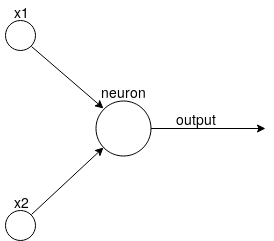
\includegraphics[width=0.25\textwidth]{images/neurons/simple_neuron.png}
    \end{center}
    \label{fig:simple-neuron}
\end{figure}
\vspace{0.25cm} \noindent
In this example our neuron \ref{fig:simple-neuron} has 2 input variables and one output, in theory it can have more or less. Furthermore Frank Rosenblatt proposes
the concept of weights for each input variable saying which variable is preferred over another one.
\vspace{0.25cm} 
\begin{figure}[H]
    \caption{Activation function of a perceptron}
    \begin{equation*}
        output=
        \begin{cases}
            0 \text{ if } \sum{_j}{w_jx_j \le threshold}\\
            1 \text{ if } \sum{_j}{w_jx_j > threshold}
        \end{cases}
    \end{equation*}
\end{figure}
\vspace{0.25cm} \noindent
A single neuron is by no means comparable to a decision making of a human being, but it can weigh variables and make decisions
by defining a threshold when a true or false should be evaluated. Another way to create a conditional behavior is to use a bias
instead of a threshold.
\vspace{0.25cm}
\begin{figure}[H]
    \caption{Neuron with bias}
    \begin{center}
        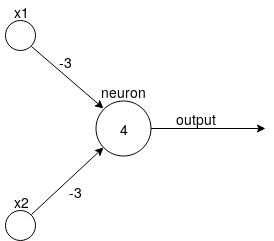
\includegraphics[width=0.25\textwidth]{images/neurons/simple_neuron_bias.png}
    \end{center} 
\end{figure}
\vspace{0.25cm}
\begin{figure}[H]
    \caption{Activation function with bias}
    \begin{equation*}
        output=
        \begin{cases}
            0 \text{ if } \sum{_j}{w_jx_j+b \le 0}\\
            1 \text{ if } \sum{_j}{w_jx_j+b > 0}
        \end{cases}
    \end{equation*}
\end{figure}
\vspace{0.25cm} \noindent
A whole network of these neurons is able to perform more complex decision making. The network \ref{fig:neural-network} is a feed forward network, but there are
bidirectional networks and even forms where the neuron passes its output back to itself. 
\vspace{0.25cm}
\begin{figure}[H]
    \caption{Example neural network}
    \begin{center}
        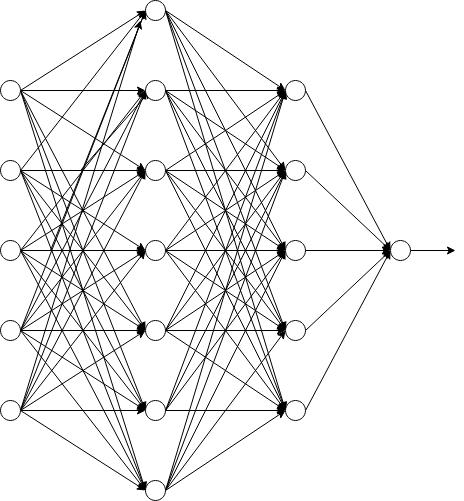
\includegraphics[width=0.5\textwidth]{images/neurons/neural_network.png}
    \end{center}
    \label{fig:neural-network}
\end{figure}
\vspace{0.25cm} \noindent
Each column in the network \ref{fig:neural-network} is called layer. The first column is referred to as the input layer and the last one as the output. All the
ones in between are called hidden layers. \\
Since the result of a perceptron can only be one or zero (true or false), one major problem which occurs when using perceptrons in more
complex neural networks is that biases and weights can have weird and unwanted effects. Making perceptrons trigger where they should not.
Thats why sigmoids were invented and they build on top of the concept of perceptrons.

\subsection{Sigmoids}
The sigmoid is a activation function which expands the functionality of a neuron. Its core difference is that the output can not only be 0 or 1
but anything in between those. Therefore 0.5234 could be a valid output of the sigmoid function. Likewise it can
have weights and biases functioning the same as it would for the perceptrons.
The core difference is the arithmetic function, called the sigmoid function or sometimes the logistic function.
\begin{figure}[H]
    \begin{equation*}
        \begin{split}
            \sigma(z) & = \frac{1}{1+e^{-z}}
        \end{split}
    \end{equation*} 
    \caption{Function for sigma}
\end{figure}
\vspace{0.25cm}
To put it more explicit with input variables, weights and bias:
\begin{figure}[H]
    \begin{equation*}
        \begin{split}
            \frac{1}{1+exp(-\sum{_j}{w_jx_j-b})}
        \end{split}
    \end{equation*}
    \caption{Explicit function for sigma}
\end{figure}
\vspace{0.25cm}
\begin{figure}[H]
\begin{center}
    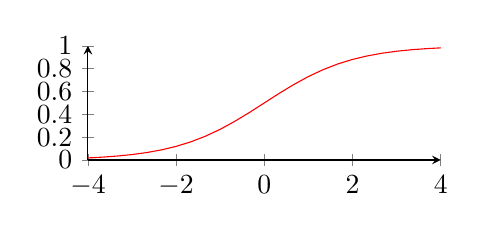
\begin{tikzpicture}
        \begin{axis}[
                width=0.5\textwidth,
                height=0.25\textwidth,
                axis x line=bottom,
                xmin=-4,
                xmax=4,
                xlabel near ticks,
                axis y line=left,
                ymin=0,
                ymax=1,
                ylabel near ticks
            ]
            \addplot[color=red, domain=-4:4, width=2] (x,{1/(1+exp(-x))});
        \end{axis}
    \end{tikzpicture}
    \caption{Graph for sigma}
\end{center}
\end{figure}
\begin{figure}[H]
    \begin{center}
    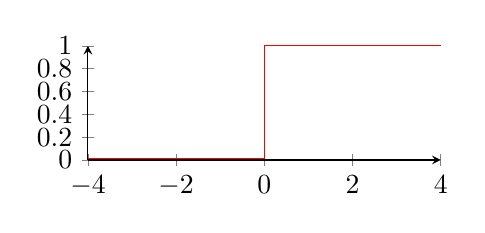
\begin{tikzpicture}
        \begin{axis}[
                width=0.5\textwidth,
                height=0.25\textwidth,
                axis x line=bottom,
                xmin=-4,
                xmax=4,
                xlabel near ticks,
                axis y line=left,
                ymin=0,
                ymax=1,
                ylabel near ticks
            ]
            \addplot[color=red, width=2] coordinates {
                    (-4,0.009)
                    (0,0.009)
                    (0,1)
                    (4,1)
            };
        \end{axis}
    \end{tikzpicture}
\caption{Graph for perceptrons}
\end{center}
\end{figure}
\vspace{0.25cm} \noindent
Since the algebraic form of {$\sigma$} is a smoothed and not step function, it makes a huge difference in the way how weight and bias influence
the activation of a neuron.

\section{Current state}
Object detection is dealing with two major problems and therefore can be split into two processes which are object localization and object
classification.  \\
There are models which have a multi layer architecture, each performing complex tasks such as analyzing, localizing and classifying each
sections individually, making the cost high and the network in general slow but accurate.
Models that combine functionality in one layer, where localization and classification is performed in one step, make the
model smaller and therefore faster but less accurate.
The balance between accuracy and speed is something that all networks deal with. Especially if the goal is to have a near real time object
detection system which is still reliable and accurate.\\
There are multiple algorithms covering various forms of this formula, called RCNN, F-RCNN, SSD, YOLO but first I will cover
the approach of detecting interesting regions in an image because this is the key problem in object detection.

\subsection{Object Localization \& Classification}
The segmentation of an image is the key approach to Object Localization and at the same time for Object Classification. Since images are
always hierarchical, meaning that each object in an image has a specific place in depth, the segmentation has to be hierarchical as well. It has to be able to cover different criteria and forms, where maybe
objects are part of a bigger total or just  smaller
objects which are inside one another. Since is not feasible to compute every possibility inside an image there has to be some kind of
separation through grids and scales. \\
As there are many approaches for analyzing and classifying regions, I am going to cover three localization algorithms which
are key for object detection.

\subsubsection{Exhaustive Search}
Since an object can be located anywhere in an image the scope to look through is enormous, making the computational cost for such a search very
expensive. To compensate for this cost most exhaustive search approaches such as the sliding window approach, have a fixed sizes and aspect
ratios for the window. Further it uses weak classifiers and economic image features such as histogram of oriented gradients
(HOG) to analyze each step.\cite{selectivesearch} \\ 
HOG approaches the problem of recognizing and detecting objects in an unknown image through corners. It analyzes the distribution and 
orientation of the corners, through which it is able to separate the image into multiple partitions or detect similar regions in different images.
Robert K. McConnell described the concept in a patent in 1986 but it became known in 2005 through a publication of Navneet Dalal and Bill
Triggs.\cite{hog}
\begin{figure}[!hbt]
    \caption{Output of a HOG algorithm}
    \begin{center}
        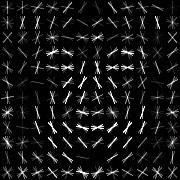
\includegraphics[width=0.3\textwidth]{images/object_detection/Dlib_Learned-HOG-Detector.jpg} \cite{hog}
    \end{center}
\end{figure}
\subsubsection{Selective Search}
A selective search algorithm is subjected into 3 design ideas:\\
\begin{itemize}
    \item Capture All Scales \\ \\
        The idea is similar to the one of the Exhaustive Search that all objects have to be found. Therefore all scales have to be
        considered as a potential region. The best approach is a hierarchical grouping, where an initial sub-segmentation has to
        be performed. \cite{selectivesearch}
        \begin{figure}[!hbt]
            \caption{Segmentation of Selective Search}
            \begin{center}
                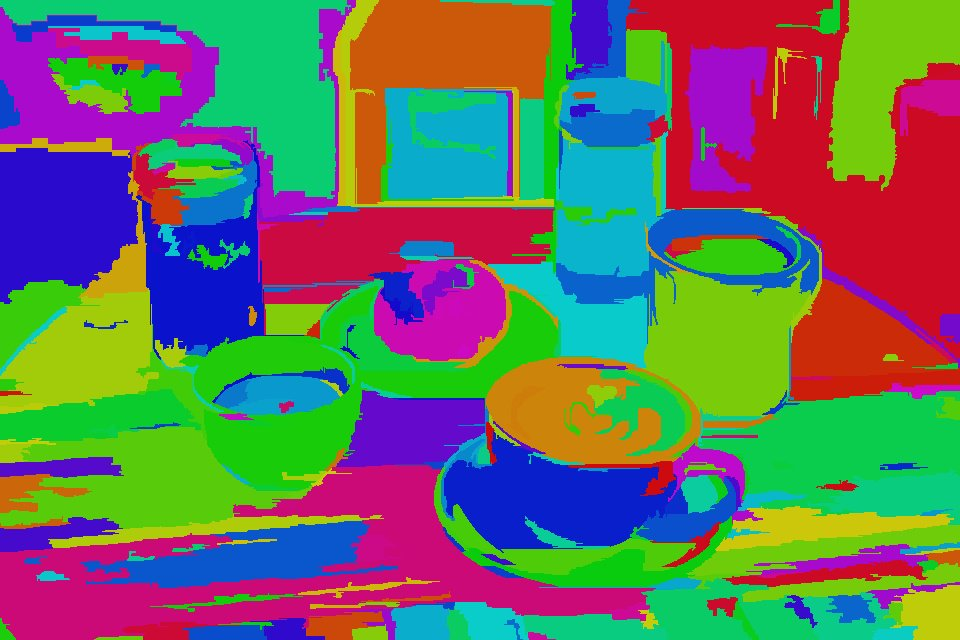
\includegraphics[width=0.5\textwidth]{images/object_detection/breakfast_fnh.jpg}\cite{sssegmentationc}
            \end{center}
        \end{figure}
        After the segmentation a grouping of regions is done by similarity. After each grouping a similarity between
        resulting regions and its neighbors are being calculated. This process is done until the whole image becomes a single region.\cite{selectivesearch}
        \begin{figure}[!hbt]
            \caption{Results of converting the segments into bounding boxes}
            \begin{center}
                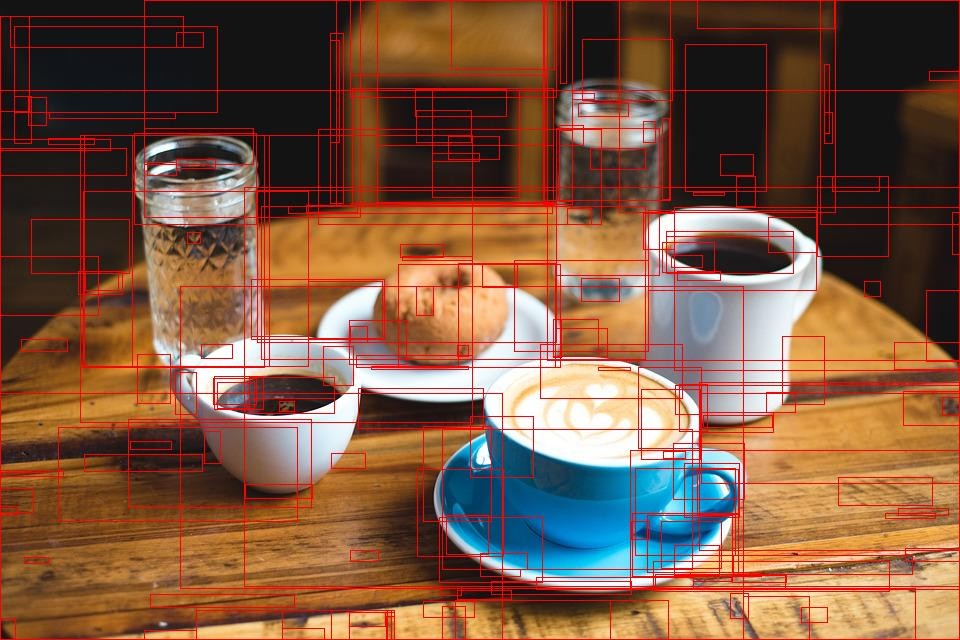
\includegraphics[width=0.5\textwidth]{images/object_detection/breakfast-top-200-proposals.jpg}\cite{sssegmentationbb}
            \end{center}
        \end{figure}
    \item Diversification \\ \\
        There is no single strategy for grouping regions together therefore multiple aspects have to be considered. Selective search
        diversifies by using a variety of color spaces with different invariance properties, by using different similarity measures and by
        varying the starting regions.  By using different color spaces, selective search is able to account for different scene and light
        conditions. To account for these variances selective search is performing the hierarchical grouping algorithm with different color
        spaces which have different invariance properties. \\
    \item Fast to Compute \\ \\
        Since each of these steps is a computation act, the main goal of this algorithm is to be fast and not create a bottleneck through its complexity.\cite{selectivesearch}
\end{itemize}
S$_{color}$: \\ \\
It measures color similarities for each region, where a color histogram of 25 bins is being created and normalized
with the L1 norm. Similarity is measured using the histogram intersection:\cite{selectivesearch} \\
\begin{center}
    \begin{equation*}
        S_{color}(r_i,r_j) = \sum_{n=1}^{n} min(c_i^{k},c_j^{k})
    \end{equation*}\cite{selectivesearch}
\end{center}
This histogram can be efficiently propagated through the hierarchy by: \\
\begin{center}
    \begin{equation*}
        \begin{split}
            C_t & = \frac{size(r_j)*C_i+size(r_j)*C_j}{size(r_i)+size(r_j)}
        \end{split}
    \end{equation*}\cite{selectivesearch}
\end{center}
S$_{texture}$: \\ \\
Selective Search measures texture similarity through the usage of the SIFT algorithm. SIFT stands for scale invariant
feature transform and is an algorithm to detect and describe features in a region. Furthermore it takes Gaussian derivatives
in eight orientations for each color channel, where a 10 bin histogram is being extracted. Similarity is measured
using the same histogram intersections and the propagation function is the same as for the color.\cite{selectivesearch}
\begin{center}
    \begin{equation*}
        S_{texture}(r_i,r_j) = \sum_{n=1}^{n} min(t_i^{k},t_j^{k})
    \end{equation*}\cite{selectivesearch}
\end{center}
S$_{size}$: \\ \\
In this step selective search encourages to merge small regions early. Doing so forces the algorithm to focus
on smaller regions which have not been merged yet first. This is encouraged because it hinders the algorithm from one
region gobbling up the rest of them one by one.\cite{selectivesearch}
\begin{center}
    \begin{equation*}
        \begin{split}
            S_{size}(r_i,r_j) & = 1 - \frac{size(r_i)+size(r_j)}{size(image)}
        \end{split}
    \end{equation*}\cite{selectivesearch}
\end{center}
S$_{fill}$: \\ \\
It measures how well region r$_i$ and r$_j$ fit into each other. The idea is to fill gaps if r{$_i$} is contained in
r$_j$, therefore it is only logical that these regions should be merged first in order to avoid holes. On the other hand
if r$_i$ and r$_j$ hardly touch each other it may form a strange region and therefore should not be merged. To keep
the process fast only the size of the regions and their contained bounding boxes are being used. Specifically the defined
BB$_{ij}$ has to be a tight bounding box around r$_i$ and r$_j$. Now S$_{fill}$ is the fraction of the image
contained in BB$_{ij}$ which is not by the regions of r$_i$ and r$_j$.\cite{selectivesearch}
\vspace{0.25cm}
\begin{center}
    \begin{equation*}
        \begin{split}
            fill(r_i, r_j) = 1 - \frac{size(BB_{ij}) - size(r_i) - size(r_j)}{size(image)}
        \end{split}
    \end{equation*}\cite{selectivesearch}
\end{center}
\vspace{0.25cm} \noindent
The final formula which measures the similarity is a combination of the above 4:
\vspace{0.25cm} \noindent
\begin{center}
    \begin{equation*}
        s(r_i,r_j) = a1s_{coulor}(r_i,r_j) + a2s_{texture}(r_i,r_j) + a3s_{size}(r_i,r_j) + a4s_{fill}(r_i,r_j)
    \end{equation*}\cite{selectivesearch}
\end{center}
\vspace{0.25cm} \noindent
\subsubsection{Region Proposal Network in Faster R-CNN}
A Region Proposal Network (RPN) takes an image of any size as an input and outputs a set of rectangular object proposals, each with an
objectness score. After the initial proposals, a sliding window is being run over the feature map. The sliding
window is of size n x n. In this example it will be of size 3 x 3. So for each sliding window a set of 9 anchors are being generated, 3
scales and 3 aspect ratios.\cite{fasterrcnn}
\vspace{0.25cm} \noindent
\begin{figure}[!hbt]
    \caption{Properties of a sliding window in RPN}
    \begin{center}
        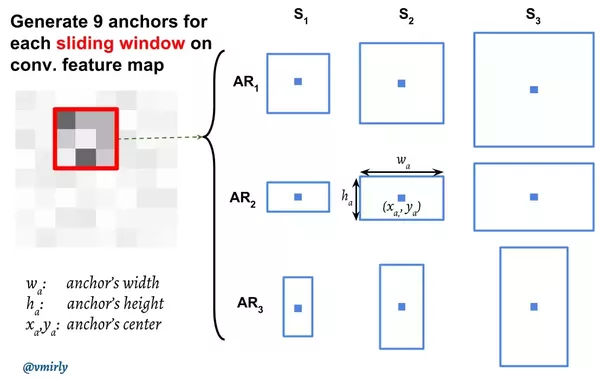
\includegraphics[width=0.5\textwidth]{images/object_detection/rpn_anchors.png}
    \end{center}
\end{figure}
\vspace{0.25cm} \noindent
Furthermore for each sliding window anchor a value called Intersection of Union short IoU is being calculated. IoU represents the value of how
much the predicted bounding box overlaps with the ground truth. The ground truth is the basis for teaching the localization network and is a
set of data predefined by a human telling the network where, which objects are in the image.\cite{fasterrcnn} \\ \\
The general idea of IoU is:
\vspace{0.25cm}
\begin{center}
    \begin{equation*}
        p =
        \begin{cases} 
            1 & \text{if IoU} > threshold \\
            -1 & \text{if IoU} < threshold \\
            0 & otherwise
        \end{cases}
    \end{equation*}
\end{center}
\vspace{0.25cm} \noindent
In the final step the results of the spatial sliding window is being fed into a smaller network which has two tasks. Classification (cls)
and regression (reg). The output of the regression represents a bounding box with (x, y, w, h). The classification value is a probability
indicating whether the bounding box contains a object or not.\cite{fasterrcnn}

\subsubsection{Single Shot Detector(SSD)}
Compared to the Faster R-CNN where the detection happens in two stages. First having the region proposal network generating proposals and
second then classifying them. SSD is a single feed forwards convolutional network to directly predict classes and anchor offsets
without requiring a second stage per-proposal.

\end{document}     
